\documentclass{standalone}
\usepackage{tikz}
\usetikzlibrary{patterns, positioning}


\begin{document}
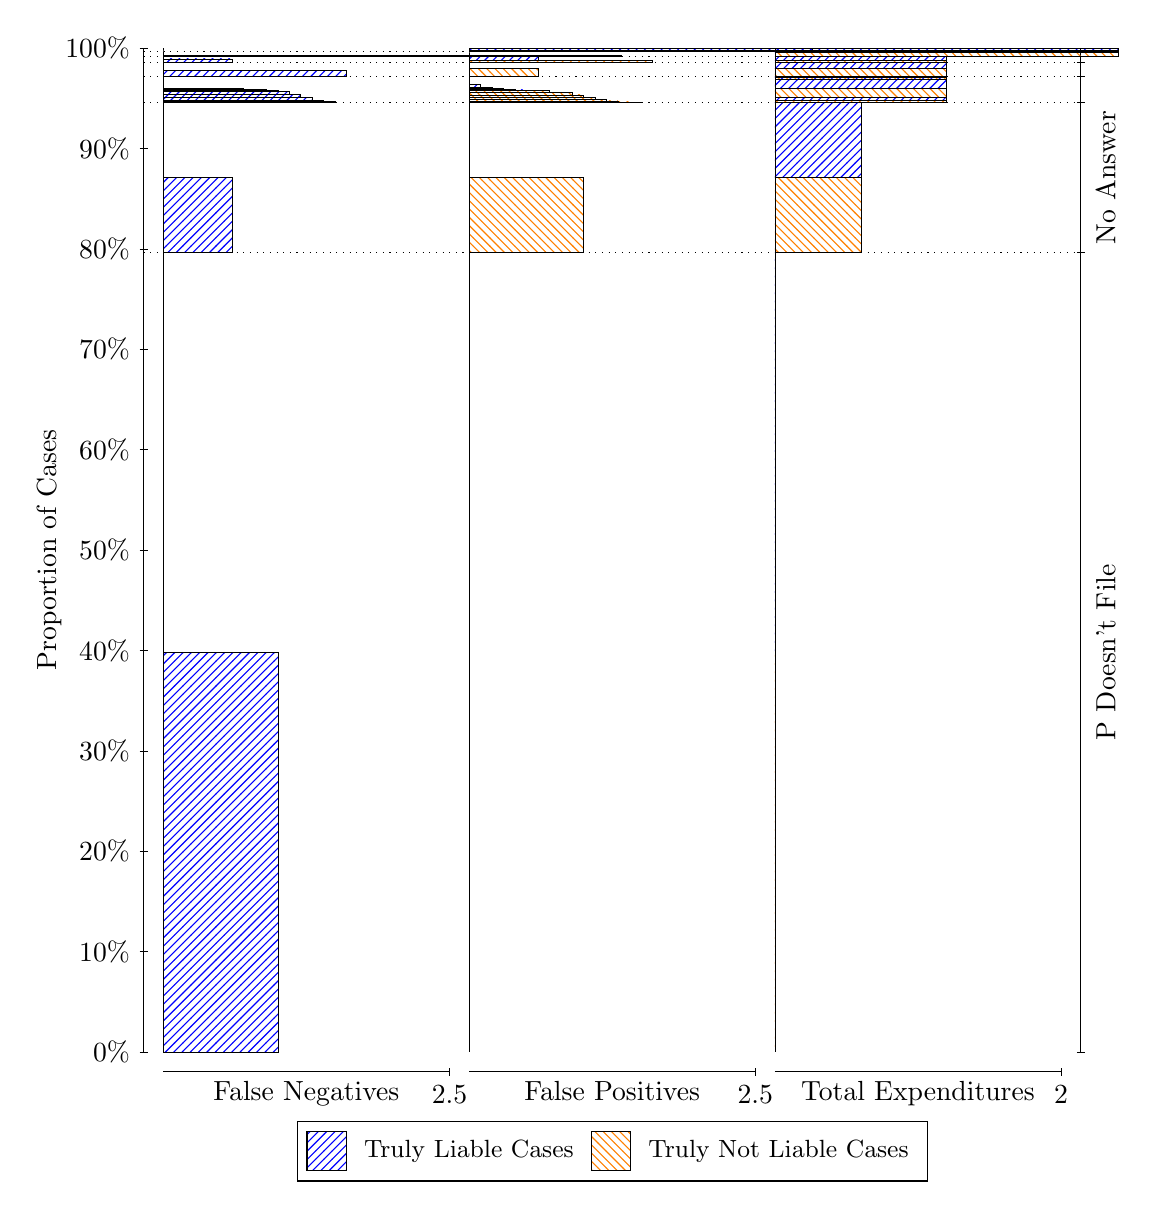
\begin{tikzpicture}
\draw[black, very thin] (1.5,1.75) -- (1.5,14.5);
\node[rotate=90, text=black, anchor=center] at (0.3, 8.125) {Proportion of Cases};
\draw[black, very thin] (1.45,1.75) -- (1.55,1.75);
\node[text=black, anchor=east] at (1.45, 1.75) {0\%};
\draw[black, very thin] (1.45,3.025) -- (1.55,3.025);
\node[text=black, anchor=east] at (1.45, 3.025) {10\%};
\draw[black, very thin] (1.45,4.3) -- (1.55,4.3);
\node[text=black, anchor=east] at (1.45, 4.3) {20\%};
\draw[black, very thin] (1.45,5.575) -- (1.55,5.575);
\node[text=black, anchor=east] at (1.45, 5.575) {30\%};
\draw[black, very thin] (1.45,6.85) -- (1.55,6.85);
\node[text=black, anchor=east] at (1.45, 6.85) {40\%};
\draw[black, very thin] (1.45,8.125) -- (1.55,8.125);
\node[text=black, anchor=east] at (1.45, 8.125) {50\%};
\draw[black, very thin] (1.45,9.4) -- (1.55,9.4);
\node[text=black, anchor=east] at (1.45, 9.4) {60\%};
\draw[black, very thin] (1.45,10.675) -- (1.55,10.675);
\node[text=black, anchor=east] at (1.45, 10.675) {70\%};
\draw[black, very thin] (1.45,11.95) -- (1.55,11.95);
\node[text=black, anchor=east] at (1.45, 11.95) {80\%};
\draw[black, very thin] (1.45,13.225) -- (1.55,13.225);
\node[text=black, anchor=east] at (1.45, 13.225) {90\%};
\draw[black, very thin] (1.45,14.5) -- (1.55,14.5);
\node[text=black, anchor=east] at (1.45, 14.5) {100\%};

\draw[black, very thin] (13.4,1.75) -- (13.4,14.5);
\draw[black, very thin] (13.35,1.75) -- (13.45,1.75);
\node[anchor=west] at (13.35, 1.75) {};
\draw[black, very thin] (13.35,11.905) -- (13.45,11.905);
\node[anchor=west] at (13.35, 11.905) {};
\draw[black, very thin] (13.35,13.807) -- (13.45,13.807);
\node[anchor=west] at (13.35, 13.807) {};
\draw[black, very thin] (13.35,14.141) -- (13.45,14.141);
\node[anchor=west] at (13.35, 14.141) {};
\draw[black, very thin] (13.35,14.313) -- (13.45,14.313);
\node[anchor=west] at (13.35, 14.313) {};
\draw[black, very thin] (13.35,14.395) -- (13.45,14.395);
\node[anchor=west] at (13.35, 14.395) {};
\draw[black, very thin] (13.35,14.456) -- (13.45,14.456);
\node[anchor=west] at (13.35, 14.456) {};
\draw[black, very thin] (13.35,14.5) -- (13.45,14.5);
\node[anchor=west] at (13.35, 14.5) {};

\draw[black, very thin, pattern color=blue, pattern=north east lines] (1.75,1.75) rectangle (3.2033,6.8273);
\draw[black, very thin, pattern color=orange, pattern=north west lines] (1.75,6.8273) rectangle (1.75,11.905);
\draw[black, very thin, pattern color=blue, pattern=north east lines] (1.75,11.905) rectangle (2.622,12.858);
\draw[black, very thin, pattern color=orange, pattern=north west lines] (1.75,12.858) rectangle (1.75,13.807);
\draw[black, very thin, pattern color=blue, pattern=north east lines] (1.75,13.807) rectangle (3.93,13.825);
\draw[black, very thin, pattern color=blue, pattern=north east lines] (1.75,13.825) rectangle (3.7847,13.835);
\draw[black, very thin, pattern color=blue, pattern=north east lines] (1.75,13.835) rectangle (3.6393,13.872);
\draw[black, very thin, pattern color=blue, pattern=north east lines] (1.75,13.872) rectangle (3.494,13.909);
\draw[black, very thin, pattern color=blue, pattern=north east lines] (1.75,13.909) rectangle (3.3487,13.947);
\draw[black, very thin, pattern color=blue, pattern=north east lines] (1.75,13.947) rectangle (3.2033,13.963);
\draw[black, very thin, pattern color=blue, pattern=north east lines] (1.75,13.963) rectangle (3.058,13.974);
\draw[black, very thin, pattern color=blue, pattern=north east lines] (1.75,13.974) rectangle (2.9127,13.979);
\draw[black, very thin, pattern color=blue, pattern=north east lines] (1.75,13.979) rectangle (2.7673,13.985);
\draw[black, very thin, pattern color=orange, pattern=north west lines] (1.75,13.985) rectangle (1.75,14.141);
\draw[black, very thin, pattern color=blue, pattern=north east lines] (1.75,14.141) rectangle (4.0753,14.217);
\draw[black, very thin, pattern color=orange, pattern=north west lines] (1.75,14.217) rectangle (1.75,14.313);
\draw[black, very thin, pattern color=blue, pattern=north east lines] (1.75,14.313) rectangle (2.622,14.361);
\draw[black, very thin, pattern color=orange, pattern=north west lines] (1.75,14.361) rectangle (1.75,14.395);
\draw[black, very thin, pattern color=blue, pattern=north east lines] (1.75,14.395) rectangle (7.5633,14.405);
\draw[black, very thin, pattern color=orange, pattern=north west lines] (1.75,14.405) rectangle (1.75,14.456);
\draw[black, very thin, pattern color=orange, pattern=north west lines] (1.75,14.456) rectangle (1.75,14.466);
\draw[black, very thin, pattern color=blue, pattern=north east lines] (1.75,14.466) rectangle (1.75,14.5);
\draw[black, very thin, pattern color=orange, pattern=north west lines] (5.6333,1.75) rectangle (5.6333,6.8274);
\draw[black, very thin, pattern color=blue, pattern=north east lines] (5.6333,6.8274) rectangle (5.6333,11.905);
\draw[black, very thin, pattern color=orange, pattern=north west lines] (5.6333,11.905) rectangle (7.0867,12.855);
\draw[black, very thin, pattern color=blue, pattern=north east lines] (5.6333,12.855) rectangle (5.6333,13.807);
\draw[black, very thin, pattern color=orange, pattern=north west lines] (5.6333,13.807) rectangle (7.8133,13.812);
\draw[black, very thin, pattern color=orange, pattern=north west lines] (5.6333,13.812) rectangle (7.668,13.817);
\draw[black, very thin, pattern color=orange, pattern=north west lines] (5.6333,13.817) rectangle (7.5227,13.829);
\draw[black, very thin, pattern color=orange, pattern=north west lines] (5.6333,13.829) rectangle (7.3773,13.844);
\draw[black, very thin, pattern color=orange, pattern=north west lines] (5.6333,13.844) rectangle (7.232,13.875);
\draw[black, very thin, pattern color=orange, pattern=north west lines] (5.6333,13.875) rectangle (7.0867,13.904);
\draw[black, very thin, pattern color=orange, pattern=north west lines] (5.6333,13.904) rectangle (6.9413,13.932);
\draw[black, very thin, pattern color=orange, pattern=north west lines] (5.6333,13.932) rectangle (6.796,13.939);
\draw[black, very thin, pattern color=orange, pattern=north west lines] (5.6333,13.939) rectangle (6.6507,13.964);
\draw[black, very thin, pattern color=blue, pattern=north east lines] (5.6333,13.964) rectangle (6.36,13.969);
\draw[black, very thin, pattern color=blue, pattern=north east lines] (5.6333,13.969) rectangle (6.2147,13.974);
\draw[black, very thin, pattern color=blue, pattern=north east lines] (5.6333,13.974) rectangle (6.0693,13.986);
\draw[black, very thin, pattern color=blue, pattern=north east lines] (5.6333,13.986) rectangle (5.924,14.002);
\draw[black, very thin, pattern color=blue, pattern=north east lines] (5.6333,14.002) rectangle (5.7787,14.04);
\draw[black, very thin, pattern color=blue, pattern=north east lines] (5.6333,14.04) rectangle (5.6333,14.141);
\draw[black, very thin, pattern color=orange, pattern=north west lines] (5.6333,14.141) rectangle (6.5053,14.237);
\draw[black, very thin, pattern color=blue, pattern=north east lines] (5.6333,14.237) rectangle (5.6333,14.313);
\draw[black, very thin, pattern color=orange, pattern=north west lines] (5.6333,14.313) rectangle (7.9587,14.347);
\draw[black, very thin, pattern color=blue, pattern=north east lines] (5.6333,14.347) rectangle (6.5053,14.395);
\draw[black, very thin, pattern color=orange, pattern=north west lines] (5.6333,14.395) rectangle (5.6333,14.446);
\draw[black, very thin, pattern color=blue, pattern=north east lines] (5.6333,14.446) rectangle (5.6333,14.456);
\draw[black, very thin, pattern color=orange, pattern=north west lines] (5.6333,14.456) rectangle (11.447,14.466);
\draw[black, very thin, pattern color=blue, pattern=north east lines] (5.6333,14.466) rectangle (9.9933,14.5);
\draw[black, very thin, pattern color=orange, pattern=north west lines] (9.5167,1.75) rectangle (9.5167,6.8274);
\draw[black, very thin, pattern color=blue, pattern=north east lines] (9.5167,6.8274) rectangle (9.5167,11.905);
\draw[black, very thin, pattern color=orange, pattern=north west lines] (9.5167,11.905) rectangle (10.607,12.855);
\draw[black, very thin, pattern color=blue, pattern=north east lines] (9.5167,12.855) rectangle (10.607,13.807);
\draw[black, very thin, pattern color=orange, pattern=north west lines] (9.5167,13.807) rectangle (11.697,13.839);
\draw[black, very thin, pattern color=blue, pattern=north east lines] (9.5167,13.839) rectangle (11.697,13.877);
\draw[black, very thin, pattern color=orange, pattern=north west lines] (9.5167,13.877) rectangle (11.697,13.986);
\draw[black, very thin, pattern color=blue, pattern=north east lines] (9.5167,13.986) rectangle (11.697,14.108);
\draw[black, very thin, pattern color=orange, pattern=north west lines] (9.5167,14.108) rectangle (11.697,14.124);
\draw[black, very thin, pattern color=blue, pattern=north east lines] (9.5167,14.124) rectangle (11.697,14.141);
\draw[black, very thin, pattern color=orange, pattern=north west lines] (9.5167,14.141) rectangle (11.697,14.237);
\draw[black, very thin, pattern color=blue, pattern=north east lines] (9.5167,14.237) rectangle (11.697,14.313);
\draw[black, very thin, pattern color=orange, pattern=north west lines] (9.5167,14.313) rectangle (11.697,14.347);
\draw[black, very thin, pattern color=blue, pattern=north east lines] (9.5167,14.347) rectangle (11.697,14.395);
\draw[black, very thin, pattern color=orange, pattern=north west lines] (9.5167,14.395) rectangle (13.877,14.446);
\draw[black, very thin, pattern color=blue, pattern=north east lines] (9.5167,14.446) rectangle (13.877,14.456);
\draw[black, very thin, pattern color=orange, pattern=north west lines] (9.5167,14.456) rectangle (13.877,14.466);
\draw[black, very thin, pattern color=blue, pattern=north east lines] (9.5167,14.466) rectangle (13.877,14.5);
\draw[black, dotted] (1.5,11.905) -- (13.4,11.905);
\draw[black, dotted] (1.5,13.807) -- (13.4,13.807);
\draw[black, dotted] (1.5,14.141) -- (13.4,14.141);
\draw[black, dotted] (1.5,14.313) -- (13.4,14.313);
\draw[black, dotted] (1.5,14.395) -- (13.4,14.395);
\draw[black, dotted] (1.5,14.456) -- (13.4,14.456);
\draw[black, very thin] (1.75,1.5) -- (5.3833,1.5);
\node[text=black, anchor=north] at (3.5667, 1.5) {False Negatives};
\draw[black, very thin] (5.3833,1.45) -- (5.3833,1.55);
\node[text=black, anchor=north] at (5.3833, 1.45) {2.5};

\draw[black, very thin] (5.6333,1.5) -- (9.2667,1.5);
\node[text=black, anchor=north] at (7.45, 1.5) {False Positives};
\draw[black, very thin] (9.2667,1.45) -- (9.2667,1.55);
\node[text=black, anchor=north] at (9.2667, 1.45) {2.5};

\draw[black, very thin] (9.5167,1.5) -- (13.15,1.5);
\node[text=black, anchor=north] at (11.333, 1.5) {Total Expenditures};
\draw[black, very thin] (13.15,1.45) -- (13.15,1.55);
\node[text=black, anchor=north] at (13.15, 1.45) {2};

\node[text=black, centered, rotate=90] at (13.72, 6.8273) {P Doesn't File};
\node[text=black, centered, rotate=90] at (13.72, 12.856) {No Answer};






\draw (7.449999999999999,1.5) node[draw=none] (baseCoordinate) {};
\begin{scope}[align=center]
        \matrix[scale=0.5, draw=black, below=0.5cm of baseCoordinate, nodes={draw}, column sep=0.1cm]{
            \node[rectangle, draw, minimum width=0.5cm, minimum height=0.5cm, pattern color=blue, pattern=north east lines] {}; &
            \node[draw=none, font=\small, text=black] (B) {Truly Liable Cases}; &
            \node[rectangle, draw, minimum width=0.5cm, minimum height=0.5cm, pattern color=orange, pattern=north west lines] {}; &
            \node[draw=none, font=\small, text=black] (B) {Truly Not Liable Cases}; \\
            };
\end{scope}

\end{tikzpicture}
\end{document}